%%%%%%%%%%%%%%%%%%%%%%%%%%%%%%%%%%%%%%%%%
% Short Sectioned Assignment
% LaTeX Template
% Version 1.0 (5/5/12)
%
% This template has been downloaded from:
% http://www.LaTeXTemplates.com
%
% Original author:
% Frits Wenneker (http://www.howtotex.com)
%
% License:
% CC BY-NC-SA 3.0 (http://creativecommons.org/licenses/by-nc-sa/3.0/)
%
%%%%%%%%%%%%%%%%%%%%%%%%%%%%%%%%%%%%%%%%%

%----------------------------------------------------------------------------------------
%	PACKAGES AND OTHER DOCUMENT CONFIGURATIONS
%----------------------------------------------------------------------------------------

\documentclass[paper=a4, fontsize=11pt]{scrartcl} % A4 paper and 11pt font size

\usepackage[T1]{fontenc} % Use 8-bit encoding that has 256 glyphs
%\usepackage{fourier} % Use the Adobe Utopia font for the document - comment this line to return to the LaTeX default
\usepackage[english]{babel} % English language/hyphenation
\usepackage{amsmath,amsfonts,amsthm} % Math packages
\newcommand\inlineeqno{\stepcounter{equation}\ (\theequation)}

\usepackage{lipsum} % Used for inserting dummy 'Lorem ipsum' text into the template

\usepackage{sectsty} % Allows customizing section commands
\allsectionsfont{\normalfont\scshape} % Make all sections centered, the default font and small caps

\usepackage{fancyhdr} % Custom headers and footers
\pagestyle{fancyplain} % Makes all pages in the document conform to the custom headers and footers
\fancyhead{} % No page header - if you want one, create it in the same way as the footers below
\fancyfoot[L]{} % Empty left footer
\fancyfoot[C]{} % Empty center footer
\fancyfoot[R]{\thepage} % Page numbering for right footer
\renewcommand{\headrulewidth}{0pt} % Remove header underlines
\renewcommand{\footrulewidth}{0pt} % Remove footer underlines
\setlength{\headheight}{13.6pt} % Customize the height of the header

\usepackage{graphicx}
\usepackage{listings} 

\numberwithin{equation}{section} % Number equations within sections (i.e. 1.1, 1.2, 2.1, 2.2 instead of 1, 2, 3, 4)
\numberwithin{figure}{section} % Number figures within sections (i.e. 1.1, 1.2, 2.1, 2.2 instead of 1, 2, 3, 4)
\numberwithin{table}{section} % Number tables within sections (i.e. 1.1, 1.2, 2.1, 2.2 instead of 1, 2, 3, 4)

\setlength\parindent{0pt} % Removes all indentation from paragraphs - comment this line for an assignment with lots of text
\usepackage[margin=1in]{geometry}
%----------------------------------------------------------------------------------------
%	TITLE SECTION
%----------------------------------------------------------------------------------------

\newcommand{\horrule}[1]{\rule{\linewidth}{#1}} % Create horizontal rule command with 1 argument of height

\title{	
\normalfont \normalsize 
\textsc{Distributed Systems} \\ [5pt] % Your university, school and/or department name(s)
\horrule{0.5pt} \\[0.2cm] % Thin top horizontal rule
\huge Coursework \\ % The assignment title
\horrule{2pt} \\[0.2cm] % Thick bottom horizontal rule
}

\author{Krzysztof Wielgo} % Your name

\date{\normalsize\today} % Today's date or a custom date

\begin{document}
\lstset{language=bash}

\maketitle % Print the title

%----------------------------------------------------------------------------------------
%	QUESTION 1
%----------------------------------------------------------------------------------------

\section{Question}
In order to find find the lattice of consistent states, first we need to assign vector clocks for each of the processes' events. This is done in the Figure \ref{q1_1}:
\begin{figure}[ht!]
\centering
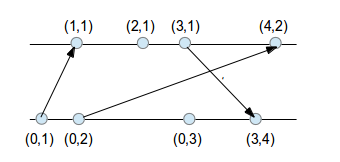
\includegraphics[width=90mm]{q1_1.png}
\caption{Vector clocks for given two processes}
\label{q1_1}
\end{figure}

Next I find all the consistent cuts for a given scenario (Figure \ref{q1_2} - dashed line depicts cuts), meaning such subset of global history for each event, which contains all the events that happened-before them.
\begin{figure}[ht!]
\centering
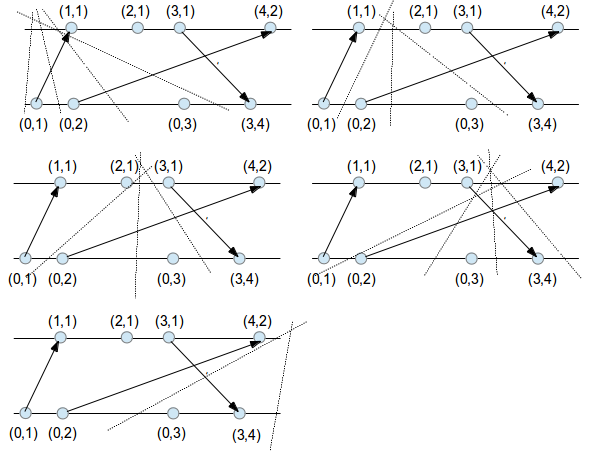
\includegraphics[width=90mm]{q1_2.png}
\caption{All possible consistent cuts for a given scenario}
\label{q1_2}
\end{figure}

This enables for creating a lattice of consistent states as in a Figure \ref{q1_3}.

\begin{figure}[ht!]
\centering
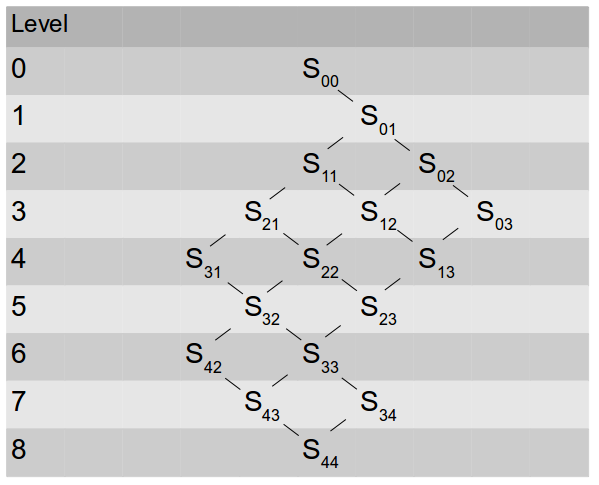
\includegraphics[width=90mm]{q1_3.png}
\caption{The lattice of global states for the execution in Figure \ref{q1_1}}
\label{q1_3}
\end{figure}


%------------------------------------------------

%----------------------------------------------------------------------------------------
%	QUESTION 2
%----------------------------------------------------------------------------------------

\section{Question}

Starvation, the possibility of indefinite postponement of entry for a process that has requested it, may occur in few systems. Examples of such systems are:
\begin{itemize}
\item central server algorithm with priorities queues - server that first serves messages with high priorities. If the client, with low priority sends a request for acquisition of mutex it may wait indefinitely if the server is busy with handling requests for higher-priority clients. The solution to this problem could be serving clients based on their priority and age of the outstanding message;
\item central server algorithm with iterative server - if the mutual exclusion server allows clients for arbitrarily long transactions (when a client is in possession of mutex), it could lead to other processes starvation. This situation happens, if the process is killed or blocked somehow (this could be solved e.g. with heartbeat messages) or malfunction; 
\item two phase locking algorithms - a type of non-blocking algorithm, which prevents from deadlock. At the first phase, process tries to acquire all the locks necessary to carry out its task. If it's not successful, it releases them and tries again after some time. This approach, however, doesn't guarantee that at any time all the mutexes will be available at the same time, what could lead to its starvation.
\end{itemize}

%------------------------------------------------
%----------------------------------------------------------------------------------------
%	QUESTION 3
%----------------------------------------------------------------------------------------

\section{Question}

To realize a given task, we need to use provided tree structure. Its execution is divided into four following steps:
\begin{itemize}
\item informing the root node $r$ about the necessity to carry out the calculation. This, however could have two different scenarios:

- if the node starting the computation is the root itself, this can be skipped. Both costs (message and time) of this operations are 0;\\
- otherwise, the request has to be delivered to the root. This is done with sending a request along $node \rightarrow parent$ paths until root is reached. In this case, the both costs for that operation equal $O(D)$, where $D$ is a diameter of the tree. The worst case scenario is when a tree is a simple chain, which would result in a complexity of $O(n-1)=O(n)$;
\item once the root knows it needs to start the computation, it starts a tree broadcast. This is realized in a following matter: 

- root sends a broadcast message to all its children;\\
- once the message is received, every other graph node forwards it to its own children;\\
- broadcast is terminated on the leaf nodes (they have no children to pass the message on).

The message complexity of this algorithm is $O(n)$ (since it's sent over n-1 spanning tree edges), assuming there is no broadcast acknowledgement (even though, if acknowledgement is for every broadcast received, then the complexity is the same). The time cost in a synchronous system is $O(D)$, since it has to reach the deepest node (which is at distance D from the root). As previously, worst case would be $O(n)$;

\item when the leaf node received the request for calculations, it starts convergecast aggregation. To realize this part of algorithm, I assume exchange of messages carrying following information:

- $MAX$, which is a maximum value of the $f$ function over all the subtree elements;\\
- $SUM$ - sum of all $f$ function values over the subtree elements;\\
- $CNT$ - number of subtree elements that were used for $SUM$ calculation.

Execution is carried out as below(see also Figure \ref{q3_1}):

- leaf node sends value of its $f$ function in $MAX$ and $SUM$ (they are calculated over only one variable), along with $CNT$ equal to 1;\\
- every other node waits for responses from each of its children node. It starts reception of messages with internal variables $p.sum=p.f$, $p.cnt=1$ and $p.max=p.f$ (to account for $p.f$ function value). Whenever child message is received sum is increased by the value of message $SUM$(p.sum += $SUM$), counter incremented ($p.cnt++$) and new maximum value estabilished ($p.max=max(p.max, MAX)$). When all the children responded, these variables are set as a message body, which is propagated up to the node's parent;
- once all the child nodes responded to the root $p_r.sum$ is the sum of all $p_i.f$ values, $p_r.cnt$ equals to the number of all network nodes and $p_r.max$ to the maximum of all $p_i.f$. In order to get an network average of the $p.f$, additional calculation is needed: $avg=p_r.sum/p_r.cnt$.

\textit{Note: }Algorithm assumed that the $SUM$ field can store arbitrarily large values and there is no overflow when summing $p_i.sum$.

The time and message complexity for the convergecast algorithm are $O(D)$ ($O(n)$ in worst case).
\item to carry out calculated information to the every network node, again a broadcast by the root node is issued ($O(D)$ complexity).
\end{itemize}

After aforementioned four steps are done, required information is knwon network-wide. Total complexity is equal to sum of the costs from particular steps, which is:
\begin{equation}
\underbrace{O(D)}_{request-to-root} + \overbrace{O(D)}^{tree-broadcast} + \underbrace{O(D)}_{convergecast} + \overbrace{O(D)}^{values-broadcast} <= O(n)
\end{equation}
\begin{figure}[ht!]
\centering
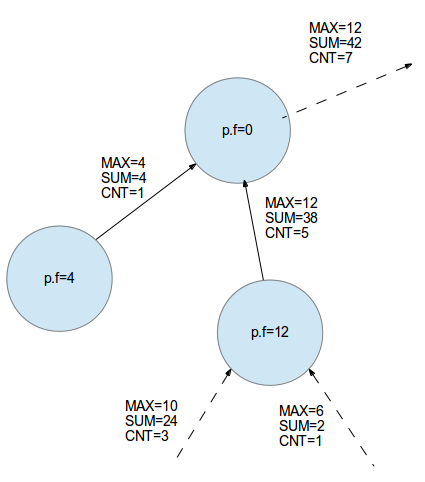
\includegraphics[width=90mm]{q3_1.png}
\caption{Example of realization of convergecast in a cut of a BFS tree}
\label{q3_1}
\end{figure}
%------------------------------------------------
%----------------------------------------------------------------------------------------
%	QUESTION 4
%----------------------------------------------------------------------------------------

\section{Question}
To find diameter of the network with weighted edges, there is a need to find shortest (weighted) paths for all the pairs of network nodes (vertices) and out of those distances choose the largest one. For simple examples, this could be done manually, but this one is already one that needs more effort. Thus, looking for a shortest path I realised with a program \textit{diameter.py} written in python (directory \textit{diameter} in a submitted source code for the first part of the assignment). The application does as follows:
\begin{itemize}
\item for every node in a graph, it uses modified version of Bellman-Ford algorithm, in order to find distances between particular node (root) and all the other ones;
\item out of those lengths it picks the largest one, which is considered to be diameter.
\end{itemize}
\textit{Note:} The algorithm given in a lecture was modified to behave well with negative weights - if a node \textit{p} took a distance from \textit{q} as the smallest one for a current run, it doesn't propagate its result to the \textit{q} in the next run. Otherwise, if the edge has negative weight, these nodes would exchange their values, leading to the result decrementing infinitely. 

The program requires appropriate input file, describing the graph - each line has following structure:
\begin{equation}
V_1 \ V_2 \ W
\end{equation}

, where $V_1$ and $V_2$ are vertices of the edge and $W$ its weight. Program takes handles directed graphs as well, so in order to describe the one given in a question, one needs to create two inputs for every edge:
\begin{equation}
\begin{matrix}
... \\
V_1 \ V_2 \ W \\
V_2 \ V_1 \ W \\
...
\end{matrix}
\end{equation}

For our particular example, the graph diameter is:
\begin{itemize}
\item for weighted case, D=8 for "m-l-h-d" path. Results given with:
\begin{lstlisting}
#PWD is diameter directory
python diameter-bf.py ./nodes.txt
\end{lstlisting}
\item for unweighed case (all W=1), D=5 and is same for paths "k-i-f-c-a-e" and "m-l-g-c-a-e". Results obtained with:
\begin{lstlisting}
#PWD is diameter directory
python diameter-bf.py ./nodes-unweighted.txt
\end{lstlisting}
\end{itemize}
%------------------------------------------------

\end{document}